%%%%%%%%%%%%%%%%%%%%%%%%%%%%%%%%%%%%%%%%%%%%%%%%%%%%%%%%%%%%%%%%%%%%%%%%%%%%%
\section{Hybrid MPI+Threads Programming}\label{sec:back-hybrid}
%%%%%%%%%%%%%%%%%%%%%%%%%%%%%%%%%%%%%%%%%%%%%%%%%%%%%%%%%%%%%%%%%%%%%%%%%%%%%

In this section we introduce the different threading modes defined by MPI for
multithreaded environments. The MPI standard provides four levels of thread safety.

\begin{figure}%[h]
  \vspace{-1.0ex}
  \hspace{0.05\columnwidth}
  \subfigure[FUNNELED.] {
    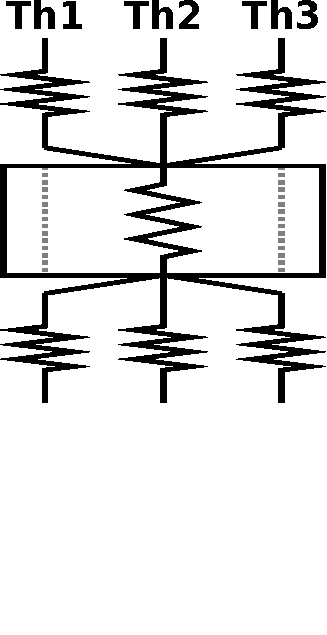
\includegraphics[width=0.26\columnwidth]{figures/mtmpi/th_funneled.pdf}
    \label{fig:th_mode_funneled}
  }
  \hspace{1.0ex}
  \subfigure[SERIALIZED.] {
    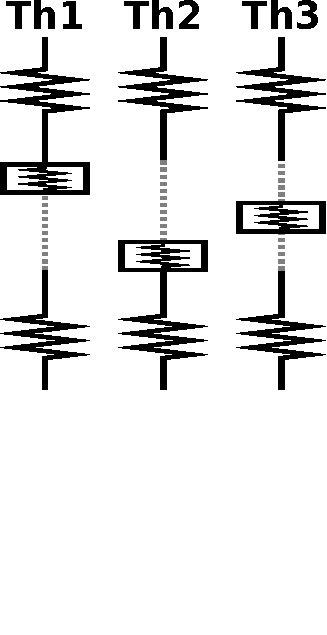
\includegraphics[width=0.26\columnwidth]{figures/mtmpi/th_serialized.pdf}
    \label{fig:th_mode_serialized}
  }
  \hspace{1.0ex}
  \subfigure[MULTIPLE.] {
    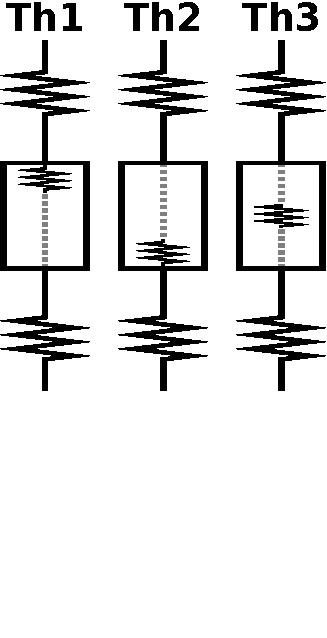
\includegraphics[width=0.26\columnwidth]{figures/mtmpi/th_multiple.pdf}
    \label{fig:th_mode_mt}
  }
  \hspace{0.05\columnwidth}
  \vspace{-2.0ex}
  \caption{Threading modes in MPI.  A line represents a thread; the
    zigzag part represents an active thread in an OpenMP region; the
    straight part represents a thread outside an OpenMP region; the
    dotted part represents an idle thread in an OpenMP region; the
    boxes represent MPI calls.}
  \label{fig:th_modes}
  \vspace{-3.0ex}
\end{figure}


\newsavebox\mpiOutsideBox
\begin{lrbox}{\mpiOutsideBox}
\begin{lstlisting}[linewidth=0.45\columnwidth]
#pragma omp parallel
{

  /* user computation */

}

MPI_Function();
\end{lstlisting}
\end{lrbox}

\newsavebox\mpiInsideMasterBox
\begin{lrbox}{\mpiInsideMasterBox}
\begin{lstlisting}[linewidth=0.45\columnwidth]
#pragma omp parallel
{
  /* user computation */
  #pragma omp master
  {
    MPI_Function();
  }
}
\end{lstlisting}
\end{lrbox}

\newsavebox\mpiInsideCriticalBox
\begin{lrbox}{\mpiInsideCriticalBox}
\begin{lstlisting}[linewidth=0.45\columnwidth]
#pragma omp parallel
{
  /* user computation */
  #pragma omp critical
  {
    MPI_Function();
  }
}
\end{lstlisting}
\end{lrbox}

\newsavebox\mpiInsideSingleBox
\begin{lrbox}{\mpiInsideSingleBox}
\begin{lstlisting}[linewidth=0.45\columnwidth]
#pragma omp parallel
{
  /* user computation */
  #pragma omp single
  {
    MPI_Function();
  }
}
\end{lstlisting}
\end{lrbox}

\begin{figure}%[h]
\vspace{-1ex}
\setlength{\subfigcapskip}{5pt}
\centering
\subfigure[Outside a parallel region] {
  \usebox\mpiOutsideBox
  \label{fig:code_hybrid_outside}
}
\hfill
\subfigure[Inside omp {\tt master} region]{
  \usebox\mpiInsideMasterBox
  \label{fig:code_hybrid_master}
}
\\
\subfigure[Inside omp {\tt critical} region]{
  \usebox\mpiInsideCriticalBox
  \label{fig:code_hybrid_critical}
}
\hfill
\subfigure[Inside omp {\tt single} region] {
  \usebox\mpiInsideSingleBox
  \label{fig:code_hybrid_single}
}
\vspace{-2.0ex}
\caption{Different use cases in hybrid MPI+OpenMP.}
\vspace{-2.5ex}
\label{fig:code_omp}
\end{figure}

\vspace{1.0ex}
\noindent\textbf{MPI\_THREAD\_SINGLE.}  In this mode, a single thread
exists in the system.  This model is commonly referred to as the
MPI-only model, where a bunch of MPI processes communicate with each
other and no threads are involved.

\vspace{1.0ex}
\noindent\textbf{MPI\_THREAD\_FUNNELED.}  In this mode, multiple
th\-reads can exist, but only the master thread (the one that
initialized MPI) is allowed to make MPI calls.  Different threads can
parallelize computational phases, but all MPI communication has to be
funneled through the main thread (see
Figure~\ref{fig:th_mode_funneled}).  In typical OpenMP environments,
this involves making MPI calls either outside the OpenMP parallel
region (Figure~\ref{fig:code_hybrid_outside}) or within OpenMP master
regions (Figure~\ref{fig:code_hybrid_master}).

\vspace{1.0ex}
\noindent\textbf{MPI\_THREAD\_SERIALIZED.}  In this mode, multiple
threads can exist, and any thread can make MPI calls but only one
thread at a time.  Different threads can parallelize computational
phases, but the threads need to synchronize in order to serialize
their MPI calls (Figure~\ref{fig:th_mode_serialized}).  In typical
OpenMP environments, this involves making MPI calls within OpenMP
critical regions (Figure~\ref{fig:code_hybrid_critical}) or single
regions (Figure~\ref{fig:code_hybrid_single}).

\vspace{1.0ex}
\noindent\textbf{MPI\_THREAD\_MULTIPLE.}  In this mode, multiple
thr\-eads can exist, and any thread can make MPI calls at any time
(Figure~\ref{fig:th_mode_mt}).  The MPI implementation is responsible
for using appropriate synchronization to protect accesses to shared
internal data structures.
\vspace{1.0ex}

%%%%%%%%%%%%%%%%%%%%%%%%%%%%%%%%%%%%%%%%%%%%%%%%%%%%%%%%%%%%%%%%%%%%%%%%%%%%%
\section{MPI One-sided Communication}\label{sec:back-rma}
%%%%%%%%%%%%%%%%%%%%%%%%%%%%%%%%%%%%%%%%%%%%%%%%%%%%%%%%%%%%%%%%%%%%%%%%%%%%%